\section{CHAPTER 10: ETP\cite{etp}}
 
\begin{figure}[h!]
    \centering
    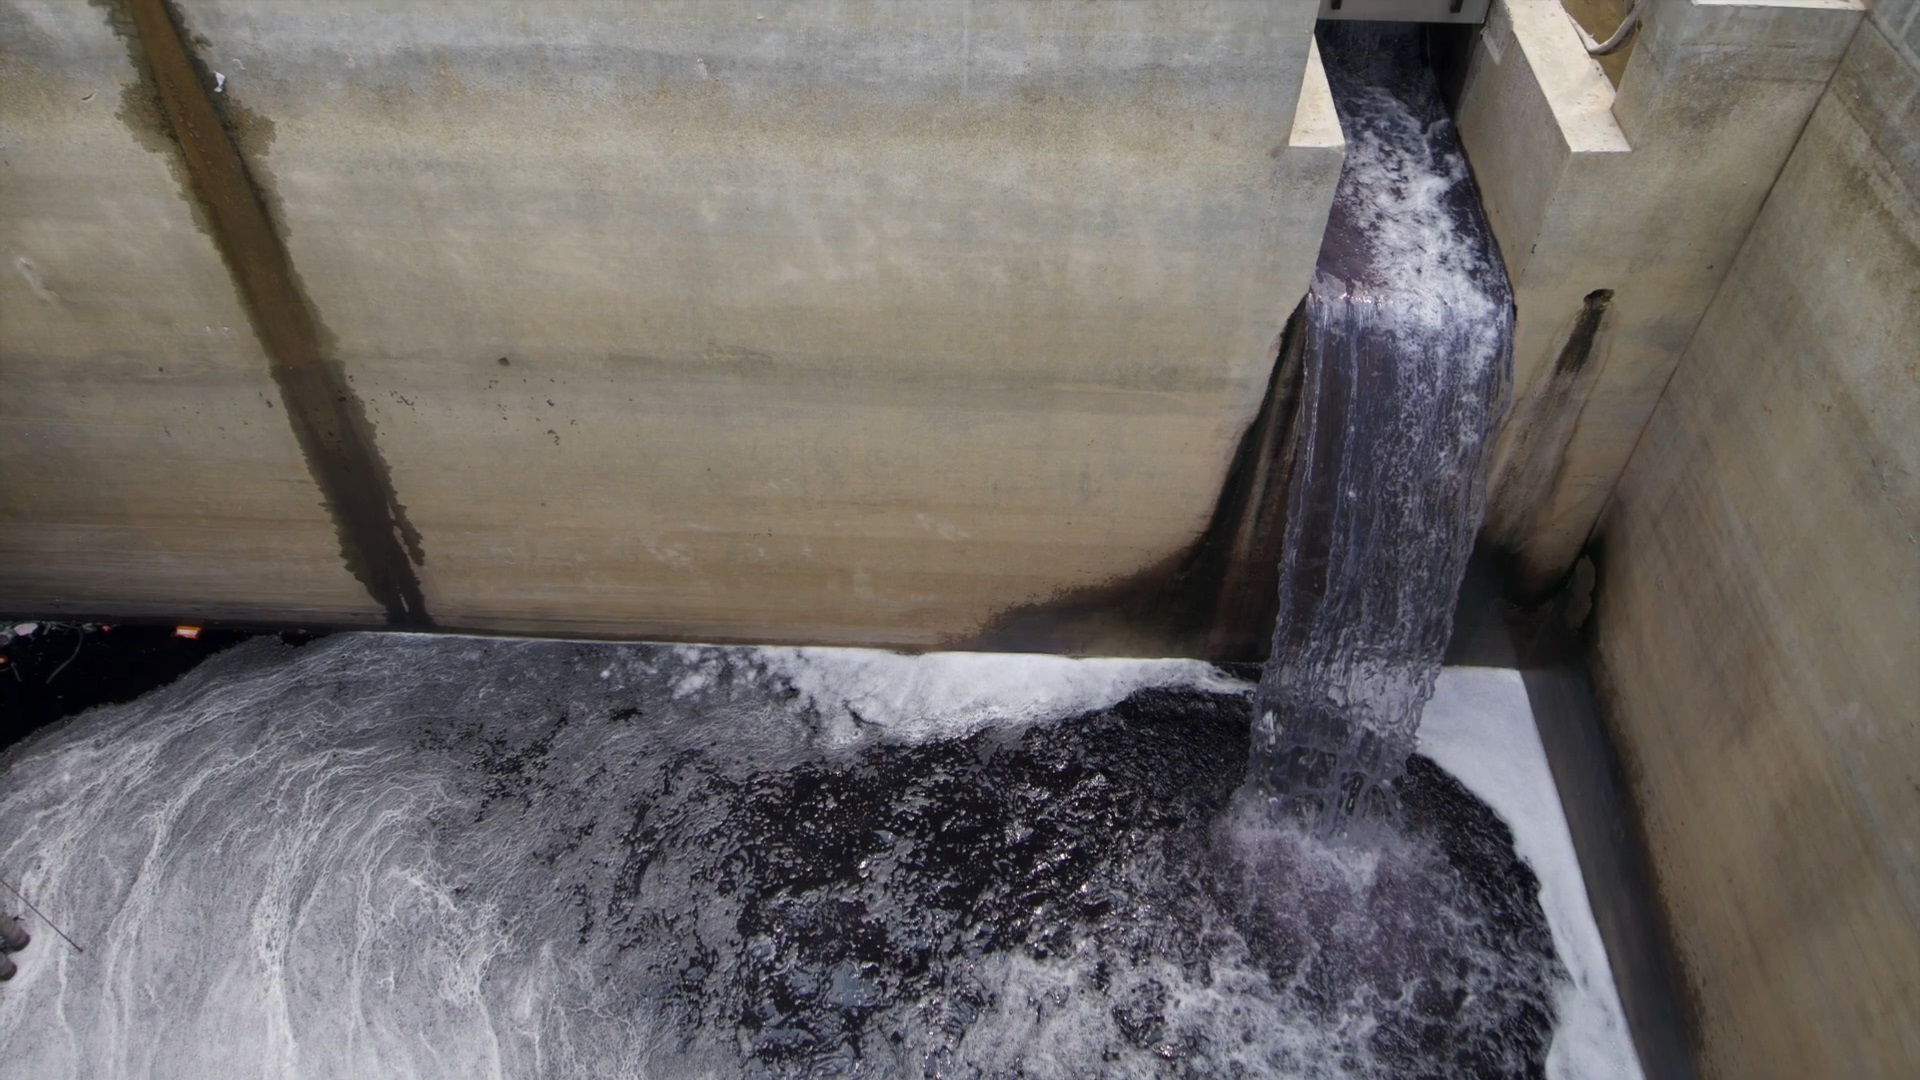
\includegraphics[width=1\linewidth]{figs/etp.jpg}
    \caption{ETP (Top) at the Industrial Tour}
    \label{fig:etp}
\end{figure}

\begin{figure}[h!]
    \centering
    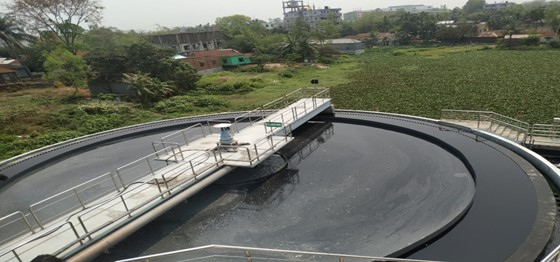
\includegraphics[width=1\linewidth]{figs/etp2.jpg}
    \caption{ETP (Bottom) at the Industrial Tour}
    \label{fig:etp2}
\end{figure}

During the visit to Forbes Marshall, the Effluent Treatment Plant (ETP) was observed as an essential system for wastewater management. The ETP process, integral to industries like pharmaceuticals, textiles, and chemicals, was demonstrated to treat highly contaminated water effectively. In this case, it was noted that Figure 39 and Figure 40 depicted biological treatment processes specifically from the textile industry.

The significant role of the ETP in managing industrial wastewater and domestic sewage was emphasized. Contaminants such as organic matter, inorganic matter, heavy metals, oil and grease, suspended particles, and other pollutants were shown to be systematically treated. Various stages of treatment were introduced to ensure the removal of impurities, including suspended particles, dissolved organic matter, and sludge disposal.

The process was described as either chemical, biological, or a combination of both methods. At Forbes Marshall, the biological type of treatment was highlighted through practical observation and explanation. The following steps were outlined as part of the wastewater treatment process:

Equalization:
The purpose of the equalization tank was explained as balancing the raw effluent from different processing units. The effluent was collected in a mixed tank and subsequently pumped into an aeration tank functioning as an equalization tank. A floating aerator was utilized to homogenize the effluent before transferring it to the neutralization tank for further treatment.

pH Control:
It was ensured that the pH value of the effluent remained within the range of 5.5 to 9.0, adhering to the standards set by the Bureau of Indian Standards (BIS). For acidic waste (low pH), bases were added to adjust the pH, while for alkaline waste (high pH), acids were employed for modification.

Coagulation:
The process of coagulation was observed, where liquid aluminium sulphate was added to untreated water. This led to the aggregation of dirt particles, forming larger, heavier particles that were easier to remove through settling and filtration.

Sedimentation:
Water movement was slowed during sedimentation, allowing heavy particles to settle at the bottom. The collected particles were referred to as sludge, which was subsequently managed in the next stages of treatment.

Filtration:
Filtration was carried out by passing water through layers of sand and gravel filters, effectively removing particulates. Regular backwashing was performed to maintain the filters’ efficiency.

Disinfection:
Before entering the distribution system, the water was disinfected. Chlorine was introduced to eliminate any remaining microorganisms, ensuring the water's safety and hygiene.

Sludge Drying:
The settled solids from sedimentation were transported to drying beds. Once the sludge thickness reached approximately 300 mm, the sludge charging was stopped, and the bed was left for natural evaporation. It was noted that the drying process typically took about 10 days.

Through this visit to Forbes Marshall, the importance of the ETP in ensuring environmentally responsible practices was highlighted. Each stage of the treatment process was carefully observed, demonstrating a commitment to sustainability and regulatory compliance in wastewater management.
\begin{figure}[h!]
    \centering
    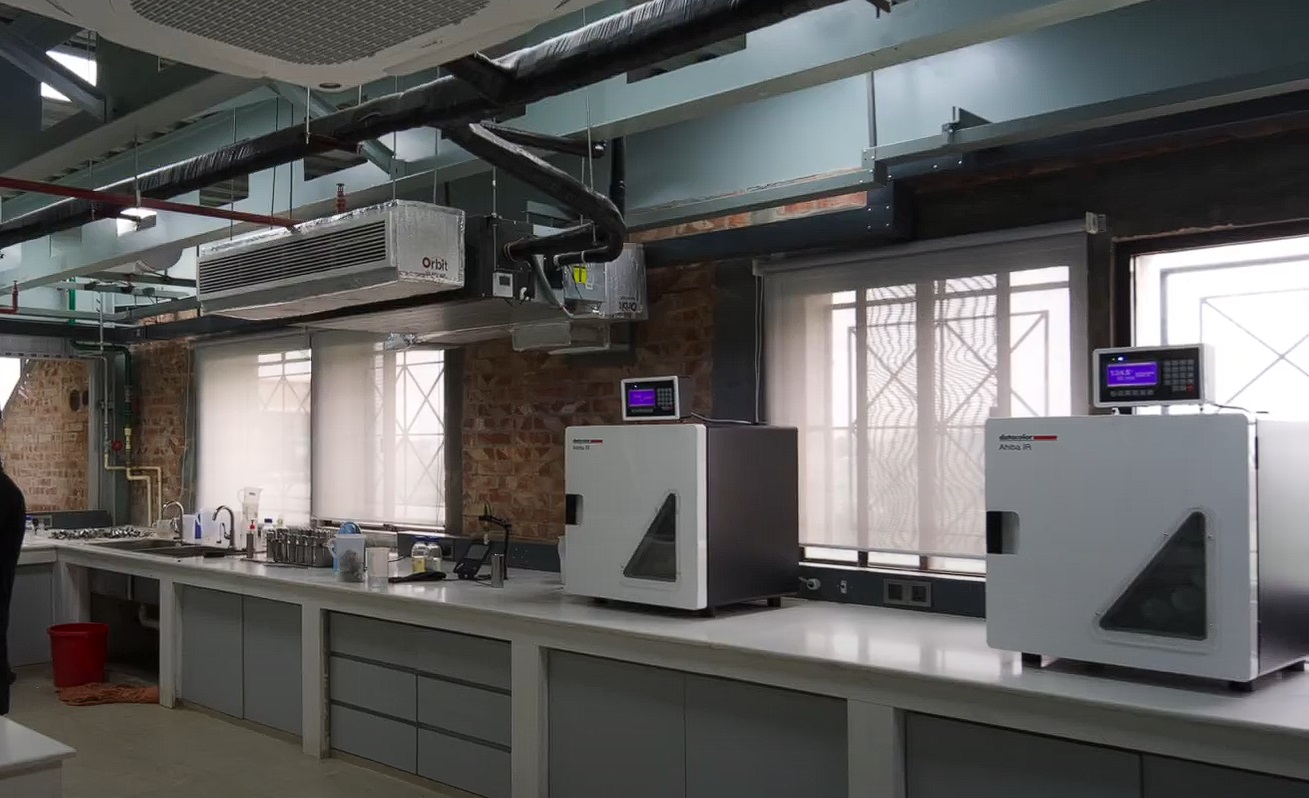
\includegraphics[width=0.8\linewidth]{figs/lab.jpg}
    \caption{LAB for measuring the condition of effluent water}
    \label{fig:LAB}
\end{figure}